\section{Carte de capteurs}\label{sec:carte-de-capteurs}

    \begin{figure}[H]
        \begin{center}
            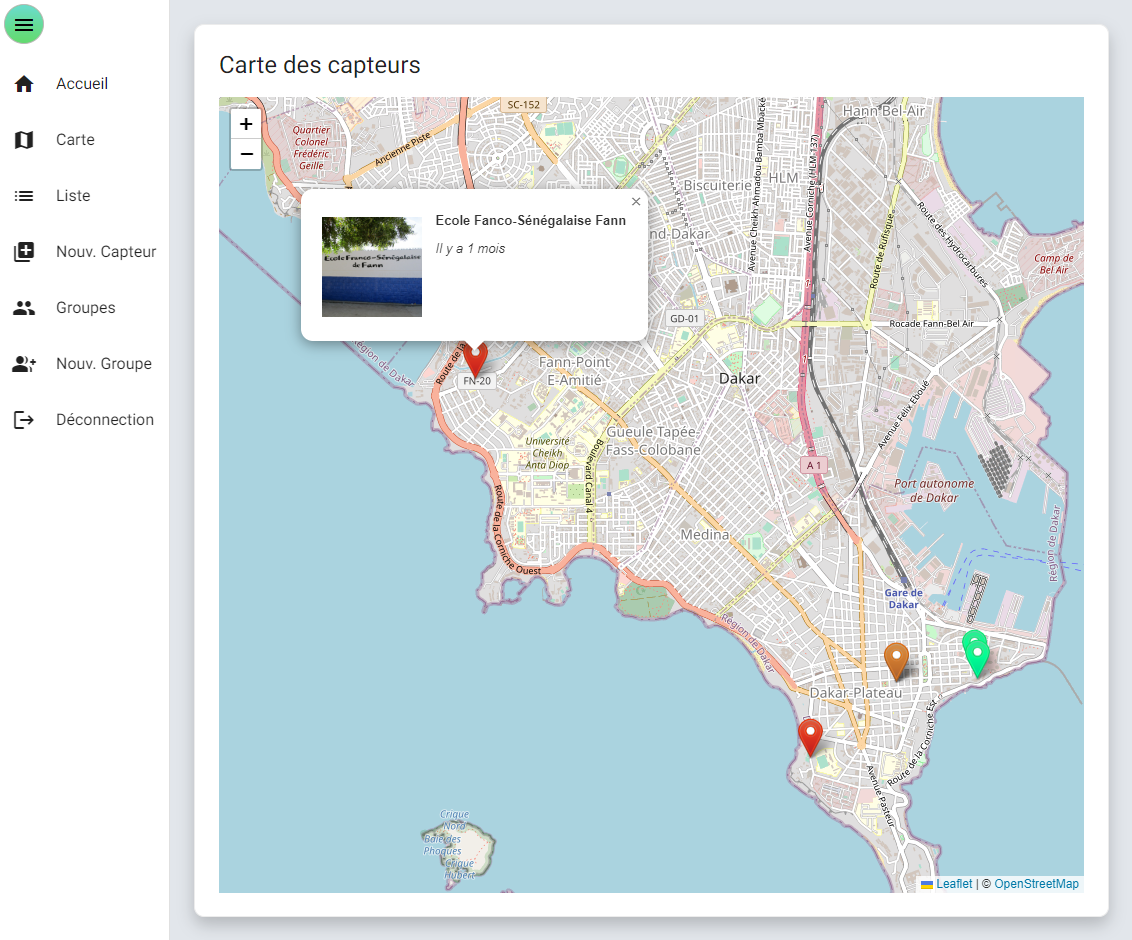
\includegraphics[width=12cm]{resources/map}
        \end{center}
        \caption{Carte de capteurs}
        \label{fig:carte-de-capteurs}
    \end{figure}

    En cliquant sur ``Carte des capteurs'' depuis la page d'accueil ou ``Carte'' dans le menu à gauche,
    vous pourrez accéder à cette page comportant une carte avec la position des capteurs.
    Chaque capteur est indiqué à l'aide d'un petit marquer.
    Il sera de couleur verte s'il a emit depuis moins d'une heure, orange s'il a été actif les dernières 24h
    et rouge si cela fait plus d'un jour qu'aucune valeur n'est émise.
    Vous pouvez aussi avoir un aperçu du capteur en le survolant avec la souris.
    Cela affichera la photo, le nom et le temps écoulé depuis la dernière émission.
    Si vous cliquez sur celui-ci, vous serez alors redirigé vers la page du capteur en question.